
\chapter{Classical numerical results and Benchmarks} % Main chapter title

\label{Chapter3} % Change X to a consecutive number; for referencing this chapter elsewhere, use \ref{ChapterX}

By last section we saw the American put was an example of an option that required numerical procedures to be priced fair. The American put is far from the only example of a derivative without a closed-form solution. In this chapter the two first sections deals with pricing American put option with 1 underlying risky asset, where in the last section we try to price options with several underlying risky assets. \\

The two first sections is two classical valuing algorithms in computational finance the Cox-Ross-Rubinstein (CRR) binomial model \parencite{CRR} and the Least Square Monte Carlo (LSM \parencite{lsm}) approach with one underlying asset. The binomial model is an example of a strategy to approximate the B-S model and the LSM is a method trying to solve the variational inequalities. We could also have chosen to solve the free boundary problem with implicit finite difference, but we chose to focus on the two other numerical procedures. The final section in this chapter will be trying to value exotic options with several underlying assets. Here we will extend the binomial pricing model to multidimensional (\parencite{NEK} and \parencite{BEG}) and provide some closed form solutions (\parencite{Johnson87} and \parencite{Ouwehand2006}). Therefore the chapter have two purposes to gain insight into valuation for exotic options and provide some benchmarks for the Neural Network in the coming chapters.

%----------------------------------------------------------------------------------------
%	SECTION 1
%----------------------------------------------------------------------------------------
\section{Cox Ross Rubenstein Model}\label{CRR}
The classical binomial model presented in this section inspired by \parencite{CRR} \parencite{Hull} \parencite{finKont} will be used for pricing an american put stock option and to build the foundation for the multidimensional binomial model \parencite{BEG}. The Binomial model provides an intuitive and easy implementable model for valuing american and european options. The binomial model comes handy, when no analytical model exists e.g. for an american put option. The Binomial model also has its limitations, because it is not suited for valuing path dependent options or options with a lot of several underlying factors. The key difference on the Binomial model and the other numerical procedures is that the binomial model is build on a discrete framework. \\

We work with the financial market $(\Omega, \mathcal{F}, \mathbb{F}, P, S_0, S_1)$, where the filtration is generated by $S_1$, $\mathbb{F}= \sigma(\mathcal{F}_{k})_{k=0,1,\ldots, T}$ and the sigma algebra is chosen to be $\mathcal{F}=\mathcal{F}_{T}$. It is well known from discrete arbitrage teory, that the binomial market model with two assets, where $u>r>d>-1$ is complete and arbitrage free model. The u,d and r describes the evolution of the discrete stochastic process for the stock and the free interest rate on the bank account. 
\begin{align*}
S_{0}(k)=S_{0}(0) \cdot \exp(\Delta t \cdot r \cdot k) \quad where \ S_{0}(0)=1\\
S_{1}(k)=S_{1}(0)\prod_{j=1}^{k} Y_{j} \quad where \ Y_1,Y_2, \ldots, Y_k \ are \ i.i.d. \ and \ S_1(0)>0
\end{align*}
We assume that the $Y_i=$\[ \begin{cases} 
      u & with \ probability \ p \\
      d & with \ probability \ (1-p)
   \end{cases}
\]
Remember that in arbitrage teory we work with the market expectation, hence we want the equivalent martingale measure. The risk neutral valuation formula holds also in discrete time:
\begin{theorem}\label{RNVF-Discrete}
\textbf{Risk-neutral valuation formula in discrete time. }
Assume there exists a risk free asset. Then the market is arbitrage free if and only if there exists a risk neutral measure $Q \sim P$ s.t.
\begin{align}
s= \exp(- r \Delta t) \cdot E^Q[S(t+\Delta t)|S(t)=s] 
\end{align}
Where $\Delta t$ is a single time-step.
\end{theorem}
From the above theorem, we can calculate the equivalent martingale measure:\\
$$q=\frac{e^{\Delta t}-d}{u-d}$$
The martingale measure q is unique in the binomial model, because it is complete. We have seen that the binomial model with the market ($S_0(k), S_1(k)$) is a arbitrage free and complete model, hence we are left with the question how to introduce a derivative with payoff $H$. The binomial model gives a recursice formula, because the filtration $\mathbb{F}$ has the structure of a binary tree. I.e. the one-step transition probabilities are the same in each node throughout the tree, because of the i.i.d. assumption.
\begin{equation}
\begin{split}
V(k-1)=\exp(-r \Delta t) (qV^{u}(k)+(1-q)V^{d}(k))\\
with \ terminal \ condition \ V(T)=H 
\end{split}
\end{equation}
The path-independence payoff for the american put makes the tree recombining, so there is only T+1 terminal nodes at maturity. If the derivative was path-dependent e.g. an asian option, then we have a non-recombinin tree and $2^{N}$ terminal nodes. This is a computational inefficient, which explains that the binomial model should not be used for path-depending derivatives. The problem with a derivative with several underlying e.g. a basket option is also the increasing number of nodes, because now you have $2^d$ possible one-step transitions.

\begin{figure}[H]
\centering
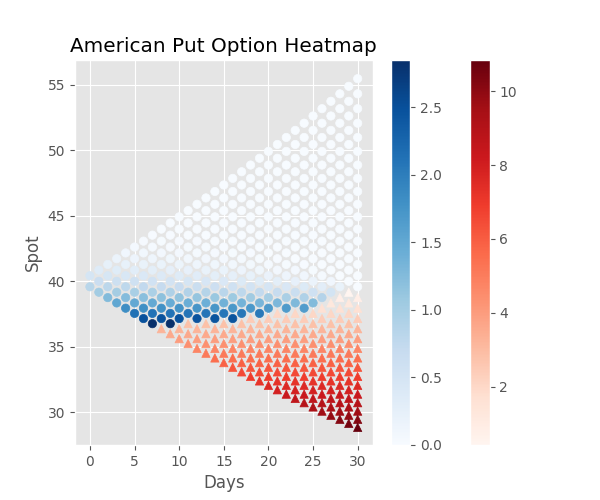
\includegraphics{Figures/BinomialTree.png}
\decoRule
\caption[Binomial Tree]{A valuation tree of an american put option price based on the binomial model, where the color indicate the value and the dots are marking the continuation nodes. The parameters are S(0)=40, N=30, $\Delta t =$ 1 day, K=40 and u=1.0106}
\label{fig:BinomialTree}
\end{figure}

To value an American put option, we lay out all the possible path of the stock based on $S_1(0),\sigma$ and $T$. First we need to construct the tree, then afterwards work backwards in the tree for valuation. Figure \ref{fig:BinomialTree} is an example of a constructed tree, where the value of the option is also included by color. To construct the tree we need to specify the number of equidistant time-steps $\Delta t$ ($\Delta t = \frac{T}{N} \ where \ N=No. \ of  \ steps$) for the tree, where for each step we add another possible value for the stock. We only add 1 more possibility for each time-step because the tree recombines.  The d and u is chosen s.t. they match volatility. So we choose:
$$u= \exp(\sigma \sqrt{\Delta t}) \quad d= \exp(-\sigma \sqrt{\Delta t})$$
For valuing an American put option, we value the exercise value at maturity (time T) for all possible outcomes for the stock. Then we use backward induction where we compare the intrinsic value with the conditional expectation, where we choose the maximum of these two. If we denote $V_{j}(k)$ as the value of the option to time $k\cdot \Delta t$ and j is the node at that time. For an put option we have at maturity:
$$V_{j}(k)=\max(K-S_1(0)\cdot u^{j} \cdot d^{N-j},0) \quad for \ j=0,1,\ldots, N \ and \ k=0,1,\ldots, T$$
At each node we compare the intrinsic value with the continuation value, where the continuation value is given for each node by the two possible one-step transitions:
$$V_{j}(k)=\exp(-r \Delta t) (q   \cdot V_{j+1}(k+1) + (1-q) \cdot V_{j}(k+1)) \quad for \ j=0,1,\ldots, N $$
Remember from above that the binomial model has a recursive structure, hence use backward induction to value the option:
$$V_{j}(k)=\max(K-S_1(0)\cdot u^{j} \cdot d^{N-j},\exp(-r \Delta t) (q   \cdot V_{j+1}(k+1) + (1-q) \cdot V_{j}(k+1))) \quad for \ j=0,1,\ldots, N$$
The first term in the max function is the intrinsic value and the second term is the condition expectation by RNVF. The comparison will be applied for every node in each time-step $\Delta t$  and all the way back in time to the initialization date. By this procedure we get present value of the American option. One design decision is to choose number of time-steps considering a trade-off between computational efficientcy and accurary. The precision for the algorithm increases with the number of steps and the option value stabilizes for increasing number of steps (see Figure \ref{fig:binConv})
\begin{figure}[H]
\centering
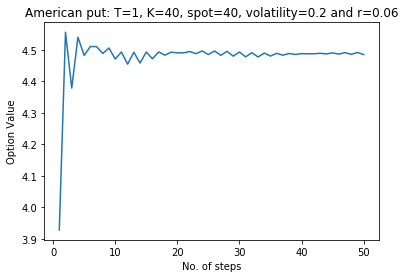
\includegraphics{Figures/binConv.png}
\decoRule
\caption[Convergence Of Binomial Model]{Price for a american put option based on the binomial model, where the independent variable is the number of time-steps. Vol. is an abbreviation for volatility.}
\label{fig:binConv}
\end{figure}
Figure \ref{fig:binConv} illustrates that around 40 steps the option value stabilizes for an option with 1 year to maturity.\\

The central concepts arbitrage and completeness from continuous time also work in the discrete time setup. The paper \parencite{CRR} which introduced the binomial model to option pricing came after the Black-Scholes model described in section \ref{Chapter2} \parencite{B-S-Paper}. The main reason for developing a model in discrete time, is that the discrete time approach gives a simplified model in terms of the mathematics and highlights the essential concepts in arbitrage theory. You can argue that the simpler mathematics in this model makes the binomial model more instructive and clear. Besides being easier to understand for non-mathematician it works nicely with other options than the european options like american options.\\

Even though we assume the stock price moves at discrete time instead in continuous time it can actually be shown for a European Option that if the number of time-steps in the tree approaches infinity. The Binomial model will then converge to the continuous time closed form solution for a European option \parencite{CRR} \parencite{Hull}. Hence the binomial pricing model will be equivalent with the continuous time analytical pricing model derived by Fischer Black and Myron Scholes in the limit for European options \parencite{CRR}. 

%----------------------------------------------------------------------------------------
%	SECTION 2
%----------------------------------------------------------------------------------------

\section{Least Square Monte Carlo Method}\label{LSM}
The classical result in this section is of a different nature, because it is based on simulation and the linear model. This section will go through the valuation method assuming 1 underlying risky asset. To price a american put options, we are faced with the optimal stopping problem:
\begin{equation}\label{optimalStopProblem}
\begin{split}
V_0 = \sup_{\tau \in \mathcal{T}(0,\ldots,T)} E\{ e^{-r \tau} \cdot \max\{K-S_{tau}, 0 \} \}
\end{split}
\end{equation}
where $V_0$ is the price and $\mathcal{T}(0,\ldots,T)$ is a class of all $(0,\ldots,T)$-valued stopping times. The stock values are modelled via black scholes theory (see path for GBM figure \ref{fig:BM}), hence the simulated evolution for the stock under the risk neutral valuation is given by:
\begin{equation*}
\begin{split}
S(t)=S(0) \cdot \exp \bigg( (r -\frac{1}{2} \sigma^2) t + \sigma W(t) \bigg)
\end{split}
\end{equation*}
The computer is discrete by nature, so we approximate the american put option with a bermudan put option. The K time points chosen between inception and maturity are equidistant time steps and by chosen K sufficient large the bermuda option approximate the american option. To solve \eqref{optimalStopProblem} backward induction is applied, where the idea like in the binomial case is to start at maturity and work backward in time. 

\begin{figure}[H]
\centering
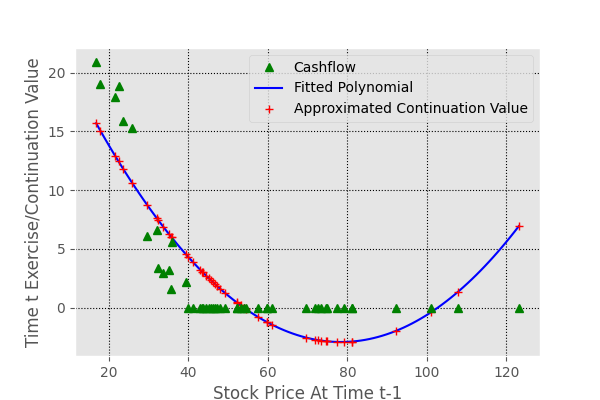
\includegraphics{Figures/LSMFit1.png}
\decoRule
\caption[Polynomial Regression Of Continuation Value]{By zooming in on a specific point of time in backward induction approach, we see how the algorithm regress the continuation value}
\label{fig:LSM1}
\end{figure}

In our setting we regress the expected payoff by continuation of the contract and compare it to the intrinsic value. The dependent variable in the regression is the expected value of continuation and the independent variables is a set of orthogonal basis functions in $L^2(\Omega, \mathcal{F}, Q)$ of the simulated paths. Typical choices for basis functions could be weighted Laguerre -, Hermit -, and Jacob polynomials. This kind of regression is a nonlinear expansion of the linear model. 

%-----------------------------------
%	SUBSECTION 1
%-----------------------------------
\subsection{LSM method for an American put}           
We want to valuate an American put option with a stock as underlying asset. We take the same assumptions as in Chapter \ref{Chapter2} (see assumption \ref{BS-Assumption}) except the option is an American option. Hence in order to simulate the paths of the stock, we simulate from a GBM: $dS(t)=rSdt + \sigma S dW_t$ where $\sigma$ and r are constant (see solution to SDE equation \ref{GBM}). We simulate 100.000 paths for the stock. Like in the binomial model, we work backward to decide the optimal stopping time. The computer is discrete, hence we simulate the stock path as an Bermudan option, where we have 50 time-steps per year. I.e. we approximate the American option with a Bermudan option on same underlying. \\

At maturity the cash flow from the option is the same as for an European put option, hence the cash flow from each path is $C(\omega,T;T, T)=max(K-S_T,0)$. We use the notation $C(\omega, s; t, T)$ denote the path of cash flows generated by the option condition on the option not being exercised before t and the option holder follow the optimal stopping strategy for all s, $t<s\leq T$.
(inspired by \parencite{lsm} p. 121). The continuation value is given by:
\begin{equation}\label{continuation-value}
\begin{split}
F(\omega; t_k)=E^Q[\sum_{j=k+1}^K \exp(-\int_{t_k}^{t_j} r(\omega,s) ds)C(\omega,t_j; t_k, T)|\mathcal{F}_{t_k}]
\end{split}
\end{equation}
where $r(\omega,t)$ is risk free interest rate, and the $\mathcal{F}_{t_k}$ is the filtration at time $t_k$.\\

We get the optimal stopping strategy by comparing thr continuation value with the intrinsic value at each time step. By working backward in time until the initialization of the option, we have approximated the the optimal stopping times and the cash flows associated with exercising at the optimal stopping times (see figure \ref{fig:LSM2}). 

\begin{figure}[H]
\centering
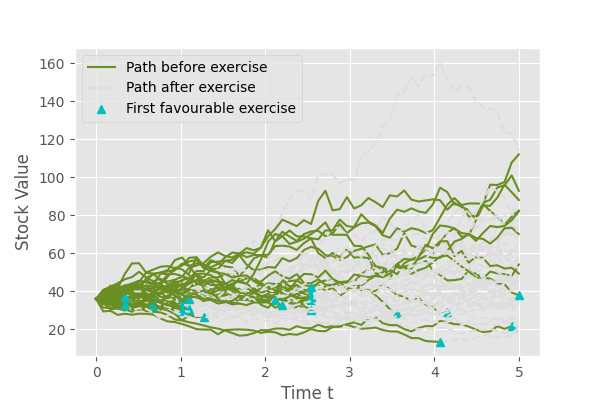
\includegraphics{Figures/LSMFit2.png}
\decoRule
\caption[Optimal Stopping Decision]{The optimal stopping decisions by the Least Square Monte Carlo Method}
\label{fig:LSM2}
\end{figure}

To estimate the condition expectation in equation \ref{continuation-value}, we regres with the basis functions taking on the underlying asset for the option being the independent variable:
$$F(\omega;t_{K-1})= \sum_{j=0}^\infty a_j L_j(X)$$
where a is the coefficients for the regression, L is the basis function, where the argument is the underlying asset $X$ \parencite{lsm}.

The LSM approach gives a lower bound for the true price of the option given optimal stopping choice:
\theoremstyle{proposition}
\begin{proposition}{}\label{BS-price-EuroCall}
\textbf{Lower Bound To True Value:} For any finite choice of M, K, and vector $\theta\in \mathbb{R}^{M \times (K-1)}$ representing the coefficients for the M basis functions at rach of the K-1 early exercise dates, let $LSM(\omega;M,K)$ denote the discounted cash flow resulting from the following the LSM rule of exercising when the immediate exercise value is positive and greater tahn or equal to $\hat{F}_{M}(\omega_{l};t_{k})$ as defined by $\theta$. Then the following inequality holds almost surely,
$$V(X)\geq \lim_{N\to \infty} \dfrac{1}{N}\sum_{i=1}^{N} LSM(\omega_i;M,K)$$
(p. 124 \parencite{lsm})
\end{proposition}

%-----------------------------------
%	SUBSECTION 2
%-----------------------------------

\subsection{Numerical results}
By the above two algorithms for valuation, we choose to vary spot, volatility and maturity for pricing an American put option with K=40 and r=0.06. This table will serve as reference for the machine learning algorithm in chapter (!TODO chapter for machine learning). For the binomial tree we use 100 time-steps, which gives stable results (compare to figure \ref{fig:binConv}) and for the LSM we use $10^5$ paths with 50 time-steps per year. The European option is valued by using BS closed form solution for a call option (see proposition \ref{BS-price-EuroCall}) and Put-call parity (see proposition \ref{Put-call-parity}).
\begin{table}[H]
\caption{Valuation of American put option with K=40 and r=0.06.}
\label{tab:treatments}
\centering
\begin{tabular}{l l l l l l l }
\toprule
\textbf{Spot} & \textbf{$\sigma$} & \textbf{T} & \textbf{Closed form European} & \textbf{Binomial Tree} & \textbf{LSM} & \textbf{abs. diff.} \\
\midrule
36 & 0.2 & 1 & 3.844 & 4.488 & 4.478 & 0.010\\
36 & 0.2 & 2 & 3.763 & 4.846 & 4.828 & 0.018\\
36 & 0.4 & 1 & 6.711 & 7.119 & 7.092 & 0.027\\
36 & 0.4 & 2 & 7.700 & 8.508 & 8.500 & 0.008\\
38 & 0.2 & 1 & 2.852 & 3.260 & 3.245 & 0.015\\
38 & 0.2 & 2 & 2.991 & 3.748 & 3.735 & 0.013\\
38 & 0.4 & 1 & 5.834 & 6.165 & 6.144 & 0.021\\
38 & 0.4 & 2 & 6.979 & 7.689 & 7.665 & 0.024\\
40 & 0.2 & 1 & 2.066 & 2.316 & 2.313 & 0.003\\
40 & 0.2 & 2 & 2.356 & 2.885 & 2.881 & 0.004\\
40 & 0.4 & 1 & 5.060 & 5.310 & 5.326 & 0.016\\
40 & 0.4 & 2 & 6.326 & 6.914 & 6.908 & 0.006\\
42 & 0.2 & 1 & 1.465 & 1.622 & 1.622 & 0.000\\
42 & 0.2 & 2 & 1.841 & 2.217 & 2.212 & 0.005\\
42 & 0.4 & 1 & 4.379 & 4.602 & 4.596 & 0.006\\
42 & 0.4 & 2 & 5.736 & 6.264 & 6.243 & 0.021\\
44 & 0.2 & 1 & 1.017 & 1.117 & 1.113 & 0.004\\
44 & 0.2 & 2 & 1.429 & 1.697 & 1.688 & 0.009\\
44 & 0.4 & 1 & 3.783 & 3.956 & 3.962 & 0.006\\
44 & 0.4 & 2 & 5.202 & 5.656 & 5.649 & 0.007\\
\bottomrule\\
\end{tabular}
\end{table}
We see the maximum difference between the two algorithms is 0.027 at S=38, $\sigma=0.4$ and T=2. The other obvious fact is that the European put has a lower value than its American counterpart, because the continuous exercise feature adds additional value to the put option. 


%----------------------------------------------------------------------------------------
%	SECTION 3
%----------------------------------------------------------------------------------------

\section{Benchmarks in higher dimensions}\label{BMHiggerDim}
In this section will we provide closed form solution for some special cases of european multivariate contingent claims. Furthermore we present a lattice approach in multidimensional for pricing both european and american multivariate contingent claims. The basic assumptions and results are given in section \ref{MultiDimModel}.

\subsection{Analytical formulas for Rainbow options}
We derive closed form solutions to european call and put options depending on several variables, for simplicity we will focus on pricing options with 2 or 3 underlying stocks. We apply the intuition given in \parencite{Johnson87} and the results given in \parencite{Ouwehand2006}. The derivatives we will consider are the geometric mean -, maximum - and minimum call option.

\subsubsection{Geometric basket call option}
For a geometric basket call option the contract function is given by:
\begin{align*}
\Phi(S(T))=\max\{ (\prod_{i=1}^{n} S_i(T))^{\frac{1}{n}}-K,0 \}
\end{align*}
The key to  derive a closed form solution is the known result that the sum of normal random variables are multivariate normal distributed.
This implies that the product of lognormal random variables are multivariate log-normal distributed. Since: 
\begin{equation*}
\begin{split}
\exp(x+y)=\exp(x)\cdot \exp(y) \\
X \sim \mathcal{N}(\mu,\sigma^2) \Rightarrow Y = \exp(X)\sim LN(\mu, \sigma^2)
\end{split}
\end{equation*}

We assume as in section \ref{MultiDimModel} that the stocks price process follows a GBM, hence:
\begin{equation}
\begin{split}
(\prod_{i=1}^{n} S_i(T))^{\frac{1}{n}} = (\prod_{i=1}^{n} S_i(0))^{\frac{1}{n}} \exp((r-\frac{1}{2n}\sum_{i=1}^{n}\sigma_i^2)T + \frac{1}{n} \sum_{i=1}^{n} \sigma_i W_i(T))
\end{split}
\end{equation}
By defining
\begin{align}
\sigma = \frac{1}{n} \sqrt{\sum_{i=1}^{n} \sigma_i^2 + 2 \sum_{i\neq j} \rho_{i,j}\sigma_i \sigma_j}\\
F=(\prod_{i=1}^{n} S_i(0))^{\frac{1}{n}} \exp((r-\frac{1}{2n}\sum_{i=1}^{n}\sigma_i^2)T + \frac{1}{2} \sigma^2 \cdot T
\end{align}
We arrive at the price by skipping some arguments:
\begin{equation}
\Pi(t,\mathcal{X})=\exp(-r*(T-t))\bigg(F N(d_1) - K N(d_2) \bigg)
\end{equation}
where $d_1=\frac{\ln(\frac{F}{K}) + \frac{1}{2} \sigma^2 T}{\sigma \cdot \sqrt{T}}$ and $d_2=d_1-\sigma \sqrt{T}$

\subsubsection{Options on the Maximum or the Minimum of Several Assets}
Here we restrict ourselves to consider the case with three underlying stocks like in \parencite{BEG} and \parencite{Ouwehand2006}, but the formula can be generalized to higher dimensions. The contract functions we consider are:
\begin{enumerate}
\item[•] Best of assets or cash: $\Phi(S(T))=\max\{S_1,S_2,\ldots,S_n,K\}$
\item[•] Call on max: $\Phi(S(T))=\max\{\max(S_1,S_2,\ldots,S_n)-K,0\}$
\end{enumerate}
We use n=3 because it shows the generality without the notation becomes to cumbersome.

We use the martingale framework developed in section \ref{MultiDimModel} to value these exotic options. The key is to choose the numeraire to a risky assets instead of the bank account. By results from section \ref{MultiDimModel} the processes are still Q-martingales given the numeraire is strictly postive. So under the asssumption the arbitrage free and complete market it follows:
$$S_0(t)E^{Q_0}_t[\frac{X_T}{S_0(T)}]=S_1(t)E^{Q_1}_t[\frac{X_T}{S_1(T)}]$$

\paragraph{Best of assets or cash}
The best of assets will both provide a price and the method for pricing call on max and min. We assume WLOG n=4 and define the payoff as for the i'th asset:
$$S_i(T) \cdot 1_{\{S_i(T)>S_j(T): i\neq j\}}$$
Hence the best of assets derivative is a sum of above equation for each asset. So we are considering four cases, because we assumed WLOG n=4. \\

For i=1 we set $S_1$ to be the numeraire asset with martingale measure $\mathbb{Q}_1$. Then we see by using RNVF (see proposition \ref{RNVF}):
\begin{equation}
\begin{split}
\Pi_1(t, \mathcal{X})&=S_1(t)E_t^{Q_1}[1_{\{S_1(T)>S_2(T), S_1(T)>S_3(T), S_1(T)>S_4(T)\}}]\\
&=S_1(t) Q_1[\ln(\frac{S_2(T)}{S_1(T)})<0, \ln(\frac{S_3(T)}{S_1(T)})<0, \ln(\frac{S_4(T)}{S_1(T)})<0]
\end{split}
\end{equation}
By cycling through the numeraires we get four derivatives that we need to add together for optaining the fair price for best of assets $\Pi_{max}(t,\mathcal{X})$. Before we can proceed we need to find the probaility under the $Q$-martingale measure. By using Ito's lemma (see \ref{Ito}):
\begin{align*}
\ln(\frac{S_i(T)}{S_j(T)})\sim \mathcal{N}(\ln(\frac{S_i(T)}{S_j(T)}) - \frac{1}{2}\sigma_{i/j}^2 \cdot (T-t), \sigma_{i/j}\sqrt{T-t})
\end{align*}
where $\sigma_{i/j}^2=\sigma_i^2+\sigma_j^2-2\rho_{ij}\sigma_i \sigma_j$.\\

Besides using the definition for $d_1$ and $d_2$ in proposition \ref{BS-price-EuroCall} we define:
\begin{align}
d^{i/j}_1 =\frac{1}{\sigma\cdot \sqrt{T-t}} \cdot \bigg( \ln(\frac{S_i}{S_j}) + \frac{1}{2} \sigma_{i/j}^2 \cdot (T-t) \bigg)\\
d^{i/j}_2=d^{i/j}_1-\sigma_{i/j} \sqrt{T-t}
\end{align}
The correlation between $\frac{S_i(T)}{S_k(T)}$ and $\frac{S_j(T)}{S_k(T)}$ is given by (see page 5 \parencite{Ouwehand2006}):
\begin{align}
\rho_{ij,k}= \frac{\rho_{ij}\sigma_i \sigma_j - \rho_{ik}\sigma_i \sigma_k - \rho_{kj}\sigma_k \sigma_j + \sigma_k^2}{\sqrt{(\sigma_i^2 + \sigma_k^2 - 2\rho_{ik}\sigma_i \sigma_k)\cdot(\sigma_j^2 + \sigma_k^2 - 2\rho_{jk}\sigma_j \sigma_k)}}
\end{align}
Hence:
$$Q_1[\ln(\frac{S_2(T)}{S_1(T)})<0, \ln(\frac{S_3(T)}{S_1(T)})<0, \ln(\frac{S_4(T)}{S_1(T)})<0]=N_3(-d_2^{2/1},-d_2^{3/1},-d_2^{4/1}, \rho_{23,1}, \rho_{24,1}, \rho_{34,1})$$
Cycling through each derivative, we get:
\begin{equation}\label{BestAsset}
\begin{split}
\Pi_{max}(t,\mathcal{X})&=S_1(t) N_3(-d_2^{2/1},-d_2^{3/1},-d_2^{4/1}, \rho_{23,1}, \rho_{24,1}, \rho_{34,1}) \\
&+S_2(t) N_3(-d_2^{1/2},-d_2^{3/2},-d_2^{4/2}, \rho_{13,2}, \rho_{14,2}, \rho_{34,2})\\
&+S_3(t) N_3(-d_2^{1/3},-d_2^{2/3},-d_2^{4/3}, \rho_{12,3}, \rho_{14,3}, \rho_{24,3}) \\
&+S_4(t) N_3(-d_2^{1/4},-d_2^{2/4},-d_2^{3/5}, \rho_{12,4}, \rho_{13,4}, \rho_{23,4})
\end{split}
\end{equation}
We can extend the above result to best of assets and cash by letting $S_4(t)=K\exp(-r(T-t))$, where K do not have any volatilty and also independent of the other assets, hence \eqref{BestAsset} becomes:
\begin{equation}\label{BestAssetOrCash}
\begin{split}
\Pi_{max}(t,\mathcal{X})&=S_1(t) N_3(-d_2^{2/1},-d_2^{3/1},d_1^{1}, \rho_{23,1}, \rho_{24,1}, \rho_{34,1}) \\
&+S_2(t) N_3(-d_2^{1/2},-d_2^{3/2},d_1^{2}, \rho_{13,2}, \rho_{14,2}, \rho_{34,2})\\
&+S_3(t) N_3(-d_2^{1/3},-d_2^{2/3},d_1^{3}, \rho_{12,3}, \rho_{14,3}, \rho_{24,3}) \\
&+K\cdot \exp(-r(T-t)) N_3(-d_2^1,-d_2^2,-d_2^3, \rho_{12}, \rho_{13}, \rho_{23})
\end{split}
\end{equation}

\paragraph{Call on max and call on min}
From \eqref{BestAssetOrCash} is easy to see the call max fair price is:
\begin{equation}\label{callMax}
\begin{split}
\Pi_{cmax}(t,\mathcal{X})&=S_1(t) N_3(-d_2^{2/1},-d_2^{3/1},d_1^{1}, \rho_{23,1}, \rho_{24,1}, \rho_{34,1}) \\
&+S_2(t) N_3(-d_2^{1/2},-d_2^{3/2},d_1^{2}, \rho_{13,2}, \rho_{14,2}, \rho_{34,2})\\
&+S_3(t) N_3(-d_2^{1/3},-d_2^{2/3},d_1^{3}, \rho_{12,3}, \rho_{14,3}, \rho_{24,3}) \\
&-K \exp(-r(T-t)) \cdot\bigg(1 - N_3(-d_2^1,-d_2^2,-d_2^3, \rho_{12}, \rho_{13}, \rho_{23})\bigg)
\end{split}
\end{equation}

To derive put max we can utilize a put-call-parity (see page 6 \parencite{Ouwehand2006}), but it takes a different form than the one presented in \ref{Chapter2} (see \ref{put-call-parity}). The relationship for the exotic call options:
$$V_c(K)+K\exp(-r\cdot (T-t)) = V_p(K)+V_c(0)$$
Where $V_c(K)$ is the value of the exotic call option.

These options will serve as benchmark for the multivariate lattice approach, and for pricing the call on min see \parencite{Ouwehand2006}.


\subsection{Lattice approach for multivariate contingent claims}
We follow the approach in \parencite{BEG} (BEG method), because it is the natural extension of the Cox Ross Rubinstein model (section \ref{CRR}) for multivariate contingent claims. The idea as in the one dimensionel case is to approximate the system of underlying processes (assumed to be GBMs) with a discrete multivariate binomial lattice. The advantage is that for exotic options like the rainbow options the valuation of european put options is readily extented to the american put options and has high accuracy. The \parencite{BEG} has its limitation in terms of number of underlyings and for path dependent options (see section \ref{CRR}), but it is very intuitive and extends easily to american options. The problem with increasing the number of underlyings is that the number of one-step transition at each node is $2^d$ and the total number of terminal nodes after N steps is $(N+1)^d$ for path-independent derivatives, which means for high dimensional problems the computational resources become an issue with this discrete approximation approach. This makes the BEG method undesirable for higher dimensions than three so we will focus on the two dimensional case. Another problem with two or more underlyings are that some one-step transition probabilities negative, which makes the model useless in those cases. \\

The model we want to approximate is the bivariate lognormal distribution, because we assume the Black Scholes model to describe the evolution of the two risky assets (section \ref{MultiDimModel}). We restrict ourselfes to the assumptions \ref{BS-Assumption} given in the classical \parencite{B-S-Paper}, hence for risk neutral pricing the SDE for the risky assets are:
$$dS_i(t)=S_i(t)r(t)dt+S_i(t)\sigma_i(t)dW^Q(t) \quad for \ i=1,2,\ldots,d$$
We divide the time from inception to maturtiy (length T) into N equidistant intervals with length $Delta t$, because we want the jump distribution to approximate the continuous time multivariate lognormal distribution. Each time interval has a jump size defined in terms of the volatility and the length of the interval:
$$u_i=\exp(\sigma_i \sqrt{\Delta t}) \quad and \quad u_i \cdot d_i = 1 \quad for \ i=1,2,\ldots,d $$
The $u_i$ and $d_i$ are the multiplication factor for the i'th stock, where the former is a jump up and the latter is a jump down for the stock. With what probability does the stock jump  up or down? This is the key in the BEG approach to approximate a multivariate lognormal distribution with a discrete distribution. The probabilities are chosen such that the characteristics functions are equal for small time steps $Delta t$ (see p. 245-246 in \parencite{BEG} for details). The probabilities for the model with two underlying risky assets:
\begin{equation}
\begin{split}
p_1=p_{uu}=\dfrac{1}{4}\bigg( 1+\rho + \sqrt{\Delta t}(\dfrac{\mu_1}{\sigma_1} + \dfrac{\mu_2}{\sigma_2}) \bigg)\\
p_2=p_{ud}=\dfrac{1}{4}\bigg( 1-\rho + \sqrt{\Delta t}(\dfrac{\mu_1}{\sigma_1} - \dfrac{\mu_2}{\sigma_2}) \bigg)\\
p_3=p_{du}=\dfrac{1}{4}\bigg( 1-\rho + \sqrt{\Delta t}(-\dfrac{\mu_1}{\sigma_1} + \dfrac{\mu_2}{\sigma_2}) \bigg)\\
p_4=p_{dd}=\dfrac{1}{4}\bigg( 1+\rho + \sqrt{\Delta t}(-\dfrac{\mu_1}{\sigma_1} - \dfrac{\mu_2}{\sigma_2}) \bigg)
\end{split}
\end{equation} 
The correlation $\rho$ between the two assets are assumed to be constant and $\mu_i=r-\frac{1}{2}\sigma_i^2$. We have illustrated below a two-dimensional lattice, where we see that the number of nodes at maturity is $(1+N)^d$.

\begin{figure}[H]
\centering
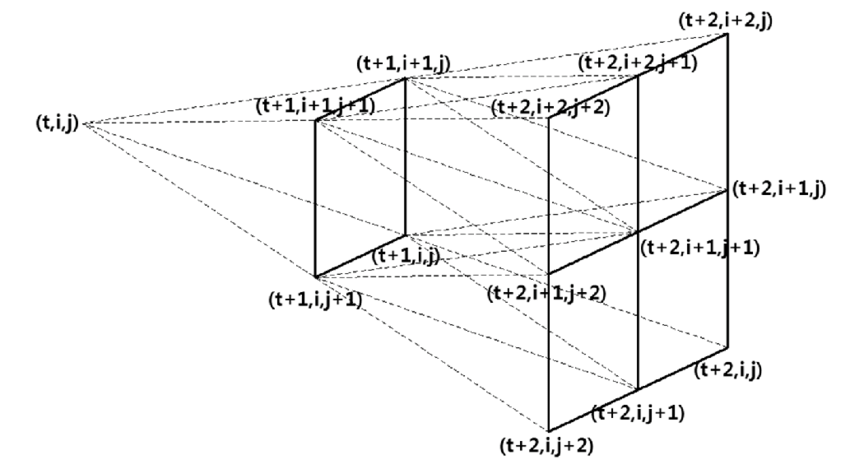
\includegraphics[width=\textwidth]{Figures/Three-dimensional-binomial-lattice.png}
\decoRule
\caption[Three Dimensionel Binomial Lattice]{Evolution of binomial model with two underlying risky asset, where t is time, i is number of up movement for $S_1$ and j is number of up movement for $S_2$  \parencite{Kim02}.}
\label{fig:threeDimLattice}
\end{figure}

After the construction of the evolution of the underlyings, we can like in the one dimensionel CRR model recursively working backward in the multidimensional binomial lattice. For the european option the recursive formula is:
$$V_{i_1,\ldots, i_d}(t)=\exp(-r\Delta t) \bigg(p_1 V_{i_1+1,\ldots, i_d +1}(t+1) + \cdots + p_{2^d} V_{i_1,\ldots, i_d}(t+1) \bigg)$$
For the american option we have the possibility of exercising between inception and maturity of the contract hence:
$$V_{i_1,\ldots, i_d}(t)=\max\{\Phi(t,\bm{S}(t)), \exp(-r\Delta t) \bigg(p_1 V_{i_1+1,\ldots, i_d +1}(t+1) + \cdots + p_{2^d} V_{i_1,\ldots, i_d}(t+1) \bigg)\}$$
With the recursive formulas we can valuate multivaraite contigent claims for a variety of exotics including the american put option with several underlying risky assets. The increasing dimensions also increase the number of one-step transition probabilities, hence the \parencite{NEK} approach (NEK) tries with setting all the probabilities equal to 0.5 and than determine the jump sizes. The NEK approach overcome the issue with negative probabilities for higher dimensions and following \parencite{NEK} the algorithm seems also to have faster convergence. The NEK and BEG approaches are both good for low dimensionel option problems, but both still suffers the curse of dimensionality. The simulations methods on the otherhand has somewhat an advantage for higher dimesions, but e.g. the LSM needed basis function grows exponential with the underlyings. We choose to present the BEG approach, because it is a natural extension of the already presented CRR model, which we already build inituition opon.\\

\subsection{Numerical And Analytical Results}
\begin{table}[H]
\caption{Valuation of multivariate contigent claims with two underlyings with K=40, $S_1(0)=S_2(0)=40$, $\sigma_1=0.2, \sigma_2=0.3$, T=1, $\rho=0.5$  and r=0.06.}
\label{tab:treatments}
\centering
\begin{tabular}{l l l l}
\toprule
\textbf{Derivative type} & \textbf{Method} & \textbf{No. Steps} & \textbf{Price} \\
\midrule
European Put Minimum & BEG & 100 & 3.790\\
& Analytic form & & \\
European Call Minimum & BEG & 100 & \\
& Analytic form & & 14.636\\
European Call Maximum & BEG & 100 & \\
& Analytic form & & 7.7996946812090755\\
American Put Minimum & BEG & 10 & 3.830\\
 &  & 50 & 3.884\\
 &  & 100 & 3.890\\
\bottomrule\\
\end{tabular}
\end{table}

